%-*-latex-*-
\chapter{Print statements and C-strings}


\textsc{Objectives}
\sidenote{
{\Large\textred{\textbf{Why the big, fat right margin? For your notes. Get busy.}}}
}
\begin{tightlist}
\li Print strings and characters using \verb!std::cout!
\li Use the \verb!\n!, \verb!\t!, \verb!\"!, \verb!\'!, 
    \verb!\\! characters
\li Use \verb!std::endl! to force newline
\li Write multiple print statements
\end{tightlist}

In this set of notes, we learn to print strings and characters.

A quick advice to ease the pain of learning your first programming language: 
Type the program 
\EMPHASIZE{exactly} as given. 
Even your spaces and blank lines must match the spaces 
and blank lines in my programs.

Let's begin ...


\newpage\section{Hello World}

Go ahead and run your first program:
\begin{console}
#include <iostream>

int main()
{
    std::cout << "Hello, world!\n";

    return 0;
}
\end{console}

{\it ... commercial break ... go to notes on software tool(s) for writing and 
running a program ...}
\sidenote{
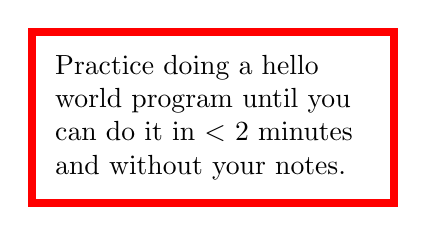
\begin{tikzpicture}
  \node[draw=red,text width=4cm,minimum height=2cm,minimum width=2cm, line width=0.1cm, inner sep=0.3cm] at (2,-2)
       {\normalsize{Practice doing a hello
         world program until you
         can do it in $<$ 2 minutes
         and without your notes.}};
\end{tikzpicture}
}

Now let's go back to the C++ code. Right now, you should think of the stuff in bold as the program:
\begin{console}[commandchars=\~\!\@]
#include <iostream>

int main()
{
    ~textbf!*** YOUR "PROGRAM" GOES HERE ***@

    return 0;
}
\end{console}


Therefore you can treat this as a template:


\sidenote{
  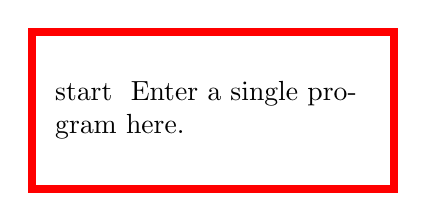
\begin{tikzpicture}
  \node[draw=red,text width=4cm,minimum height=2cm,minimum width=2cm, line width=0.1cm, inner sep=0.3cm] (a) at (2,-2) 
       {\tikzmark{start} \normalsize{ Enter a single program  here.}};
\end{tikzpicture}
}
\begin{console}[commandchars=\~\!\@]
#include <iostream>

int main()
{

    *** PROGRAM *** ~tikzmark!end@

    return 0;
}
\end{console}
\DrawArrow[red, thick]{start}{end}
\begin{console}[commandchars=\~\!\@]
#include <iostream>

int main()
{

    *** PROGRAM *** ~tikzmark!endArrow@
    
    return 0;
}
\end{console}
\sidenote{TODO ... Put your program here }

I will not explain things like 
\lq\lq \verb!#include <iostream>!'' or 
\lq\lq\verb!int main()!'' until later. 
(Technically, they are also part of  the program.)



Try this
\begin{console}
#include <iostream>

int main()
{
    std::cout << "Hello ... world! ... mom!\n";

    return 0;
}
\end{console}

%%-*-latex-*-

\begin{ex} 
  \label{ex:prob-00}
  \tinysidebar{\debug{exercises/{disc-prob-28/question.tex}}}

  \solutionlink{sol:prob-00}
  \qed
\end{ex} 
\begin{python0}
from solutions import *
add(label="ex:prob-00",
    srcfilename='exercises/discrete-probability/prob-00/answer.tex') 
\end{python0}


\begin{ex} 
\label{sec:hellodrliow}
(Go to Solution \ref{sec:hellodrliow_soln} 
on page \pageref{sec:hellodrliow_soln}) 
\\
Write a program that gets the computer to greet you:
\begin{console}
hello dr. liow, my name is c++.
\end{console}
(replace my name with yours ...  you're probably not 
\lq\lq\verb!dr. liow!'').
2.5 minutes!
\qed
\end{ex}


\begin{ex}
\label{sec:debughelloworld}
(Go to Solution \ref{sec:debughelloworld_soln} 
on page \pageref{sec:debughelloworld_soln}) 
\\
Debug (i.e., correct) this program by hand 
and then verify by running it 
with your C++ compiler.
3 minutes!
\begin{console}
#include (iostream)

int main()
(
    std;;cout < "Hello, world!\n";

    return 0;
)
\end{console}
\qed
\end{ex}



\newpage\textsc{Solutions}

\begin{soln}\label{sec:hellocolumbia_soln}
(Go to Exercise \ref{sec:hellocolumbia} on page \pageref{sec:hellocolumbia})
\begin{console}
#include <iostream>

int main()
{
    std::cout << "hello columbia\n";

    return 0;
}
\end{console}
\end{soln}


\begin{soln}
\label{sec:hellodrliow_soln} 
(Go to Exercise \ref{sec:hellodrliow} 
on page \pageref{sec:hellodrliow})
\begin{console}
#include <iostream>

int main()
{
    std::cout << "hello dr. liow, my name is c++.\n";  
 
    return 0;   
}  
\end{console}   
\end{soln}  


\begin{soln} 
\label{sec:debughelloworld_soln} 
(Go to Exercise \ref{sec:debughelloworld} 
on page \pageref{sec:debughelloworld})
\begin{console}[commandchars=\~\@\$]
#include ~underline@<$iostream~underline@>$

int main()
~underline@{$
    std~underline@::$cout <~underline@<$ "Hello, world!\n";

    return 0;
~underline@}$
\end{console}
\end{soln}








\newpage\section{Statement}

Here's the first jargon. Look at our program again:
\begin{console}[commandchars=\~\%\@]
#include <iostream>

int main()
{
    ~textbf%std::cout << "Hello, world!\n";@

    return 0;
}
\end{console}

The line in bold is a 
\EMPHASIZE{statement}. 
In C++, statements must terminate with a 
\EMPHASIZE{semi-colon}. 
Note that the semi-colon is part of the statement. 

At this point you should think of a statement as something that will cause 
your computer to perform some operation(s) when you run the program.

If you like, you can think of a statement as a sentence and the semicolon as a
period. When you're told to write a C++ statement, don't forget the 
semicolon!!! 
That would be like writing a sentence without a period (or question mark or 
exclamation mark) in an english essay.


\begin{ex}
\label{sec:nosemicolon}
(Go to Solution \ref{sec:nosemicolon_soln} 
on page \pageref{sec:nosemicolon_soln}) 
\\
Modify your program by removing the first semicolon to get this:
\begin{console}
#include <iostream>

int main()
{
    std::cout << "Hello, world!\n"

    return 0;
}
\end{console}
Run it. 
Does it work? 
Fix it. 
Test to make sure it works (that means: run the program.)
\qed
\end{ex}


\begin{ex}
\label{sec:period}
(Go to Solution \ref{sec:period_soln} 
on page \pageref{sec:period_soln}) 
\\
Replace the semicolons by periods.
\begin{console}
#include <iostream>

int main()
{
    std::cout << "Hello, world!\n".

    return 0.
}
\end{console}
Run it. Does it work? Fix it.
\qed
\end{ex}

See what I mean by this advice:

\begin{itemize}
\item[]
\textit{A quick advice to ease the pain of learning your first programming 
language: Type the program 
\EMPHASIZE{exactly} as given. 
Even the spaces and blank lines must match my programs.}
\end{itemize}

Computers are dumb (and picky about details.) 
We are the smart ones. So … when you communicate with your computer, 
you have to be exact and explicit in your programs.


\begin{ex} 
\label{sec:print}
(Go to Solution \ref{sec:print_soln} 
on page \pageref{sec:print_soln}) 
\\
Now write a program that prints any message 
(example: \lq\lq do you want green eggs and ham?'') ... 
close your notes first. Peek at your notes only when you have problems.
\qed
\end{ex}



\newpage\textsc{Solution}

\begin{soln}
\label{sec:nosemicolon_soln} 
(Go to Exercise \ref{sec:nosemicolon} 
on page \pageref{sec:nosemicolon})
\\
No it won't work. 
You must have the semicolon.
\qed
\end{soln}


\begin{soln}
\label{sec:period_soln} 
(Go to Exercise \ref{sec:period} 
on page \pageref{sec:period})
\\
Nope. It won't work either. 
You \textit{must} have the semicolon.
\qed
\end{soln}


\begin{soln}
\label{sec:print_soln} 
(Go to Exercise \ref{sec:print} 
on page \pageref{sec:print})
\begin{console}
#include <iostream>

int main()
{
    std::cout << "do you want green eggs and ham?\n";

    return 0;
}
\end{console}
\qed
\end{soln}





\newpage\section{C-Strings}

The stuff in quotes is called a C-string or just a string:
\begin{console}
#include <iostream>

int main()
{
    std::cout << "Hello, world!\n" ;

    return 0;
}
\end{console}

You can think of a string as textual data. 
(Soon I'll talk about numeric data for numeric computations. 
Got to have that for computer games, right?)

Double quotes are used to mark the beginning and ending of the string. 
So technically they are not part of the string. 
That's why when you run the above program, you do not see double-quotes.


\begin{ex} \label{sec:string_without_delimiters}
(Go to Solution \ref{sec:string_without_delimiters_soln})
Does it work without the double-quotes?
\begin{console}
#include <iostream>

int main()
{
    std::cout << Hello, world!\n;

    return 0;
}
\end{console}
\qed
\end{ex}

In the string 
\verb@"Hello, world!\n"@, 
\verb!H! is a character. 
The next character is \verb!e!. Etc. 
When we talk about characters we enclose them with single-quotes. 
So I should say character \verb!'H'! rather than 
\verb!H! or \verb!"H"!. 
You can think of the character as the smallest unit of data in a string. 

The string \verb@"Hello, world!\n"@ contains characters 
\verb!'H'! and \verb!'e'! and \verb!'l'! and \verb!'l'! and 
... 
However a character such as 
\verb!'H'! can contain one and only one unit of textual data. 
So you cannot say that \verb!'Hello'! is a character. 

Note that a string can contain as many as characters as you like: 
10, 20, 50, 100, etc. 
There's actually a limit, but we won't be playing around with a string with 
1,000,000 characters anyway for now --
that would be a pain to type!!! 
Note that a string can contain no characters at all: 
\verb!""!. 
Of course a string can contain exactly one character. 
For instance, here's a string with one character: \verb!"H"!. 

Note that \verb!"H"! is a string with one character whereas 
\verb!'H'! is a character. 
You just have to look at what quotes are used to tell if the thingy is a 
string or a character. That's all.


\begin{ex} \label{sec:string_delimiter_using_single_quotes} 
(Go to Solution \ref{sec:string_delimiter_using_single_quotes_soln})
Does it work with single-quotes?
\begin{console}
#include <iostream>

int main()
{
    std::cout << 'Hello, world!\n';

    return 0;
}
\end{console}
\qed
\end{ex}


\begin{ex} \label{ex:print_character}
(Go to Soluton \ref{soln:print_character})
Can you also print characters?? (You did think about this, right?) Try this:
\begin{console}
#include <iostream>

int main()
{
    std::cout << '?';

    return 0;
}
\end{console}
\qed
\end{ex}


\begin{ex} \label{soln:find_string_character}
(Go to Solution \ref{ex:find_string_character})
Which of the following is a string, a character, or neither:
\begin{verbatim}
    "I"      
    like     
    {eggs}   
    "and"    
    'ham'    
    '.'      
\end{verbatim}
\qed
\end{ex}


\newpage
\textsc{Solution}

\begin{soln} \label{sec:string_without_delimiters_soln}
(Go to Exercise \ref{sec:string_without_delimiters})
No!
\qed
\end{soln}

\begin{soln} \label{sec:string_delimiter_using_single_quotes_soln}
(Go to Exercise \ref{sec:string_delimiter_using_single_quotes})
No!
\qed
\end{soln}

\begin{soln} \label{soln:print_character}
(Go to Exercise \ref{ex:print_character})
Yes.
\qed
\end{soln}

\begin{soln} \label{ex:find_string_character}
(Go to Exercise \ref{soln:find_string_character})
Which of the following is a string, a character, or neither:
\begin{verbatim}
    "I"      string
    like     neither
    'green'  neither
    {eggs}   neither
    "and"    string
    'ham'    neither
    '.'      character
\end{verbatim}
\qed
\end{soln}



\newpage\section{Case Sensitivity}

Is C++ case sensitive?

\begin{ex}
Modify your program by changing \verb!std! to \verb!Std!:
\begin{console}
#include <iostream>

int main()
{
    Std::cout << "Hello, world!\n";

    return 0;
}
\end{console}
Run it. Does it work? Fix it.
\qed
\end{ex}

\begin{ex}
Modify your program by changing \verb!return! to \verb!RETURN!:
\begin{console}
#include <iostream>

int main()
{
    std::cout << "Hello, world!\n";

    RETURN 0;
}
\end{console}
Does it work? Fix it.
\qed
\end{ex}


Now answer this question:

Is C++ case sensitive? Circle one: \,\,\, YES  \,\,\, NO

(duh ... I'm not taking answers in class.)






\newpage\section{Whitespaces}

A whitespace is ... well ... a white space.

Spaces, tabs, and newlines are whitespaces.


\begin{ex}
Modify your program by inserting some spaces:
\begin{console}
#include <iostream>

int main()
{
    std::cout            << "Hello, world!\n";

    return 0;
}
\end{console}
Does it work?
\qed
\end{ex}

\begin{ex}
Modify your program by inserting some newlines:
\begin{console}
#include <iostream>

int main()
{
    std::cout << 




            "Hello, world!\n";

    return 0;
}
\end{console}
\qed
\end{ex}



In general you can insert whitespaces between 
\lq\lq basic words'' understood by C++. 
These \lq\lq basic words'' are called \textbf{tokens}. 
(Oooooo another big word.)

If you think of statements as sentences, 
semi-colons as periods, then you can think of tokens as words.


For instance the following are some tokens from the above program: 
\texttt{int}, \texttt{return} and even \texttt{\{}.

We say that C++ \textbf{ignores whitespace}. 


\begin{ex}
Try this:
\begin{console}
#include <iostream>

int main()
{
    std :: cout << "Hello, world!\n";

    return 0;
}
\end{console}
Does it work?
Now try this:
\begin{console}
#include <iostream>

int main()
{
    std:     :cout << "Hello, world!\n";

    return 0;
}
\end{console}
Does it work?
\qed
\end{ex}



The above 
shows you that \textbf{::} is a token – you cannot break it down.


\begin{ex}
Try this:
\begin{console}
#include <iostream>

int main()
{
    std    ::    cout << "Hello, world!\n";

    return 0;
}
\end{console}
Does it work?
\qed
\end{ex}


Try this:
\begin{console}
#include <iostream>

int main()
{
    std::cout << "Hello,          world!\n" ;

    return 0;
}
\end{console}


The whitespaces between tokens are removed when your computer runs your C++ program. So, to the computer, it doesn't matter how much whitespace you insert between tokens -- it still works.

However spaces in a \textit{\textbf{string}} 
are not removed before the program runs. 
The space characters \texttt{' '}
(there are 10 in the above string) are actually characters within the string.

Note that although you can insert whitespaces, 
in general, good spacing of a program makes it easier to read. 
Therefore you must follow the style of spacing shown in my notes. 
In particular, I 
\EMPHASIZE{don't} want to see monstrous programs like this 
(although the program does work):
\begin{console}
#include <iostream>

int                        main(){std
::
                    cout<<

"Hello, world!\n"; return 0; }
\end{console}
or this: 
\begin{console}
#include <iostream>
int main(){std::cout<<"Hello, world!\n";return 0;}
\end{console}
And don't try to be cute this like ...
\begin{console}
#include <iostream>
int
 main
  ()
   {
    std
     ::
      cout
       <<
        "Hello, world!\n"; 
         return 0; 
          }
\end{console}
The above examples are excellent candidates for the F grade. 
The correct coding style produces this:
\begin{console}
#include <iostream>

int main()
{
    std::cout << "Hello, world!\n";

    return 0;
}
\end{console}

The left trailing spaces of a statement is called the 
\EMPHASIZE{indentation} 
of the statement:
\begin{console}
#include <iostream>

int main()
{
    std::cout << "Hello, world!\n";
    TODO: left-right red arrow for indentation
 
    return 0;
}
\end{console}
\sidenote{
TODO ...
Indentation. 
}
It's a common programming style to use 4 spaces for indentation. 








\newpage\section{Special characters}


Hmmmm ... you don't see the \verb!\n! printed out. In fact what's it for???

Try this:
\begin{console}
#include <iostream>

int main()
{
    std::cout << "Hello, \nworld!\n";

    return 0;
}
\end{console}
And this
\begin{console}
#include <iostream>

int main()
{
    std::cout << "Hel\nlo, \nworld!\n";

    return 0;
}
\end{console}
And finally this:
\begin{console}
#include <iostream>

int main()
{
    std::cout << "Hello, world!";

    return 0;
}
\end{console} 
So you can think of the print cursor as jumping to the next line whenever a 
\verb!\n! is encountered. 

As a matter of fact you cannot separate the 
\verb!\! from the \verb!n!. 
\verb!\n! is consider \textit{\textbf{one}} single character. 
So technically I should write \verb!'\n'!. 
\verb!'\n'! is called the 
\EMPHASIZE{newline character}.




\begin{ex} 
Write a program that prints this:
\begin{console}
^ ^
0 0
 |
---
\end{console}
\qed
\end{ex}



Try this:
\begin{console}
#include <iostream>

int main()
{
    std::cout << "1\t2\tbuckle my shoe\n3\t4\t...\n";

    return 0;
}
\end{console}

The \verb!'\t'! move the print cursor to the next tab position. 
\verb!'\t'! is also a character. 
It's called the \textbf{tab character}.

Special characters like the above (the newline and the tab characters) are not printable and so we have to use some special notation to say 
\lq\lq the newline character'' or the 
\lq\lq the tab character''. 
Computer scientists decided (long time ago) to use 
\verb!\! to indicate a special character. 
These are called \textbf{escape characters}.

Now recall that \verb!"! is used to mark the beginning and end of a string. What if you want to print something like this:
\[
	\texttt{.....".....}
\]
Try this:
\begin{console}
#include <iostream>

int main()
{
    std::cout << ".....".....";

    return 0;
}
\end{console}
Doesn't work right? Do you see why?

Now try this:
\begin{console}
#include <iostream>

int main()
{
    std::cout << "He shouted, \"42!\"\n";

    return 0;
}
\end{console}

So in a string, \verb!\"! will let you print \verb!"!. 

\verb!'\"'! is actually a character. 
There are two \verb!'\"'! characters in the above string  
\verb@"He shouted, \"42!\"\n"@.


\begin{ex}
Write a program that prints this:
\begin{console}
She said, "I would rather marry a pig."
\end{console}
\qed
\end{ex}

\begin{ex}
Write a program that prints this:
Here's a standard formula:
\begin{console}
       2      2          2
(x + y)   =  x  + 2xy + y
\end{console}
There are two \verb!' '! characters on each side of the 
\verb!'='! character.
\qed
\end{ex}


\begin{ex}
Write a program that prints this:
\begin{console}
 d  3     2
-- x  = 3x
dx
\end{console}
\qed
\end{ex}


\begin{ex}
How would you print the character \verb!'!. Let me tell you that
\begin{console}
std::cout << ''';
\end{console}
won't work.
\qed
\end{ex}



\begin{ex}
Write a program that print the backslash character, i.e. \verb!\!.
\qed
\end{ex}

\begin{ex}
Write a program that prints this:
\begin{console}
He said, "I am! I'm a pig! Really!"
\end{console}
\qed
\end{ex}



\begin{ex}
Write a program that prints this:
\begin{console}
Get the Gold!
+-------------+
|             |
| --------+ | |  
|         | | |
| +---+ | | | |
| |G  | | |   |
| +-+ +-+ | | |
| | |       | |
| | +-----+-+ |
|               <---
+-------------+
\end{console}
\qed
\end{ex}


\begin{ex}
Write a program that prints this:
\begin{console}
#include <iostream>

int main()
{
    std::cout << "Hello, world!\n";

    return 0;
}
\end{console}
\qed
\end{ex}


The number of characters is a string is called 
\EMPHASIZE{length}
of the string. For instance the string 
\begin{verbatim}
                    "Hello, world!\n"
\end{verbatim}
has a length of 14. 


\begin{ex}
What is the number of characters (i.e., the length) of the following strings?
\begin{tightlist}
\li \verb!"columbia"!
\li \verb!""!
\li \verb!"columbia,mo"!
\li \verb!"columbia, mo"!
\li \verb@"ma ma mia!"@
\li \verb@"ma ma mia!\n"@
\li \verb@"ma\tma\tmia!\n\n"@
\end{tightlist}
\qed
\end{ex}


(You'll see much later that in every string, there's actually an extra secret character. This is however not included in the count of the length of the string. Don't worry about this for now. I will be coming back to this later.)









\newpage\section{Printing More than One Strings or Characters}

Try this
\begin{console}
#include <iostream>

int main()
{
    std::cout << "Hello, " << "world!\n";

    return 0;
}
\end{console}
And this:
\begin{console}
#include <iostream>

int main()
{
	std::cout << "Hello, " << "world!\n"
                  << "Spam, \n";

	return 0;
}
\end{console}
And this:
\begin{console}
#include <iostream>

int main()
{
	std::cout << "Hello, " << "world!\n"
                  << "Ham, " << "eggs! \n";

	return 0;
}
\end{console}
And this:
\begin{console}
#include <iostream>

int main()
{
	std::cout << "Hello, " << "world!\n"
                  << "Ham, " << "e" << "ggs! \n";

	return 0;
}
\end{console}

By the way you should try this:
\begin{console}
#include <iostream>

int main()
{
    std::cout << "a" << "" << "b";

    return 0;
}
\end{console}

\verb!""! 
is an 
\EMPHASIZE{empty string} 
(also called a null string): 
it's a string with no characters.


\begin{ex}
The output of the following program:
\begin{console}
#include <iostream>

int main()
{
    std::cout << "ham", "and", "eggs"
              << "\n";
      
    return 0;
}
\end{console}
is
\begin{console}
ham and eggs
\end{console}
True or false? (Verify with your C++ compiler.)
\qed
\end{ex}


\begin{ex}
The output of the following program:
\begin{console}
#include <iostream>

int main()
{
    std::cout << "ham" << "and" << "eggs"
              << "\n";
      
    return 0;
}
\end{console}
is
\begin{console}
ham and eggs
\end{console}
True or false? (Verify with your C++ compiler.)
\qed
\end{ex}


Of course you can also print multiple characters. Try this:
\begin{console}
#include <iostream>

int main()
{
    std::cout << 'H' << 'a' << 'm' << '\n';
         
    return 0;
}
\end{console}

Here's a tiring hello world program:
\begin{console}
#include <iostream>

int main()
{
    std::cout << 'H' << 'e' << 'l' << 'l' << 'o'
              << ',' << ' ' 
              << 'w' << 'o' << 'r' << 'l' << 'd' 
              << '!' 
              << '\n';
         
    return 0;
}
\end{console}

You can also mix printing strings and characters in a single statement:
\begin{console}
#include <iostream>

int main()
{
    std::cout << "Hel" << 'l' << "o, " 
              << 'w' << "orld!\n';
         
    return 0;
}
\end{console}







\newpage\section{Another Way to Go to the Next Line}

Let's go back to our hello world program:
\begin{console}
#include <iostream>

int main()
{
    std::cout << "Hello, world!\n";

    return 0;
}
\end{console}
Run yours and make sure there are no errors.

First let's make a separate string out of the newline character:
\begin{console}
#include <iostream>

int main()
{
    std::cout << "Hello, world!" << "\n";

    return 0;
}
\end{console}
Run it and make sure the effect is still the same.

Now do this:
\begin{console}
#include <iostream>

int main()
{
    std::cout << "Hello, world!" << std::endl;

    return 0;
}
\end{console}
Run it.

The \verb!std::endl! acts like a newline character. 
It's actually more than that. 
We'll talk about this when we talk about files. 
Anyway for the time being just remember that 
\verb!std::endl! forces a newline when you print it.


\begin{ex}
Read this program and, without running it, write down the output in the 
grid provided below. Once you're done writing down the output, run the program and verify that you output from reading the program matches the output you get when running the program.
\begin{console}
#include <iostream>

int main()
{
    std::cout << "Lives: 3" << std::endl
              << "Energy: 15000" << std::endl
              << "Score: 0" << std::endl;

    return 0;
}
\end{console}
Output (one per character):
\begin{python}
from latextool_basic import *
print consolegrid(numrows=5)
\end{python}
\end{ex}








\newpage\section{Multiple Statements}

\begin{ex}
Run this program
\begin{console}
#include <iostream>

int main()
{
    std::cout << "1!\n";
    std::cout << "2!\n";

    return 0;
}
\end{console}
\end{ex}


This tells you that you can have 
\EMPHASIZE{more than one statement}
in your program. (Actually the \verb!return 0;! is also a statement, but we'll ignore that for now.)

Furthermore C++ executes from 
\EMPHASIZE{top to bottom}
(at least right now!)


\begin{ex}
The following program has three print statements: 
\begin{console}
#include <iostream>

int main()
{
    std::cout << "Hello World! ";
    std::cout << "I'm the queen of England. ";
    std::cout << "I have 3 arms.";

    return 0;
}
\end{console}
Run it. Rewrite it so that it has only one print statement. 
\qed
\end{ex}


\begin{ex}
True or False? The output of this program (when you run it of course)
\begin{console}
#include <iostream>

int main()
{
    std::cout << "this is the last line\n";
    std::cout << "this is the second line\n";
    std::cout << "this is the first line\n";

    return 0;
}
\end{console}
is
\begin{console}
this is the first line
this is the second line
this is the last line
\end{console}
\qed
\end{ex}


\begin{ex}
Continuing with the previous program, 
rewrite it so that each sentence is printed on a separate line; use only one statement.
\qed
\end{ex}



\newpage\section{The \texttt{using namespace std} business}

Instead of our hello world program:
\begin{console}
#include <iostream>

int main()
{
    std::cout << "Hello, world!\n";

    return 0;
}
\end{console}
in many books you will see this:
\begin{console}
#include <iostream>
using namespace std;

int main()
{
    cout << "Hello, world!\n";

    return 0;
}
\end{console}

All the 
\begin{console}[frame=none]

        using namespace std;

\end{console}
does is that after it, instead of
\begin{console}[frame=none]

        std::cout

\end{console}
you can write
\begin{console}[frame=none]

        cout

\end{console}
i.e. without the 
\begin{console}[frame=none]

	std::

\end{console}
That's all. I'll talk about 
\lq\lq namespaces'' later 
(actually much, much, much later ... in CISS245). 
So don't worry too much about it. 


\begin{ex}
Does the following program work?
\begin{console}
#include <iostream>
using namespace std;

int main()
{
    cout << "Hello, world!" << endl;

    return 0;
}
\end{console}
\qed
\end{ex}


So not only can you replace \verb!std::cout! with cout after doing the 
\begin{console}[frame=none]

    using namespace std;

\end{console}
you can also replace \verb!std::endl! with \verb!endl!.





\newpage\section{Summary}

A \textbf{statement} 
is something that will cause your computer to perform some operation(s). 
In C++ statements must terminate with a semi-colon.

C++ is case-sensitive. 

C++ ignores whitespace (between tokens).

Something that looks like 
\verb@"Hello, World!\n"@ 
(i.e. characters within double quotes) is called a 
\textbf{string} or a 
\textbf{C-string}.

A \textbf{string} is either empty (the null string), 
i.e. \verb!""!, or it is made up of characters. 
For instance the first character of the string
\begin{console}[frame=none]
 
    "Hello, World!\n"

\end{console}
is \verb!'H'!.

There are special characters: 
\verb!'\n'! causes the cursor to jump to a new line while 
\verb!'\t'! moves to the next tab position, 
\verb!'\"'! is the double-quote character, 
and \verb@'\''@ is the single-quote character. 
The backslash character is \verb@'\\'@. 
These are called \textbf{escape characters}.

To print a string, you execute the following statement:
\begin{console}[frame=none, commandchars=\~\!\@]

        std::cout << ~textit![some string]@;

\end{console}
You can print more than one string in a single print statement:
\begin{console}[frame=none, commandchars=\~\!\@]

        std::cout << ~textit![string1]@ << ~textit![string2]@
                  << ~textit![string3]@ << ~textit![string4]@;

\end{console}
Printing one or more characters is the same:
\begin{console}[frame=none, commandchars=\\\{\}]

        std::cout << \textit{[some character]};
        std::cout << \textit{[character1]} << \textit{[character2]}
                  << \textit{[character3]} << \textit{[character4]};

\end{console}

You can mix print strings and characters. For instance
\begin{console}[frame=none, commandchars=\\\{\}]

        std::cout << \textit{[some character]}
	          << \textit{[some string]};

\end{console}
or
\begin{console}[frame=none, commandchars=\\\{\}]

        std::cout << \textit{[some string]}
	          << \textit{[some character]};

\end{console}
You can force a newline by printing \verb!std::endl!:
\begin{verbatim}
        std::cout << std::endl;
\end{verbatim}



If your program has two or more statements like this:
\begin{console}[frame=none, commandchars=\\\{\}]

        \textit{[statement 1]};
        \textit{[statement 2]};
        \textit{[statement 3]};

\end{console}
then C++ executes top to bottom (for now).





\newpage\section{Exercises}


1. Write a C++ program that produces the following output:
\begin{console}
"Prediction is very difficult, 
especially about the future."
    Niels Bohr
    Danish physicist (1885 - 1962)
\end{console}
Use one print statement.

2. True or false: The output of 
\begin{console}
#include <iostream>

int main[]
{
    std::cout << "To be ..."
              << "or not to be ..."
              << "That" << "is the question." 
              << std::endl

    return 0
}
\end{console}
is
\begin{console}
To be ...  
or not to be ... 
That is the question.
\end{console}
Verify with your C++ compiler.


3. Find and correct 
all the error in this program (without using your C++ compiler):
\begin{console}
#include <<iostream>>

int main[]
{
    std::cout >> "Hello!/n"
    std::cout >> "I’m the king of Spain./n"
    std::cout >> "And I have 3 arms." >> std::end

    return 0
}
\end{console}
The expected output is
\begin{console}
Hello!
I'm the king of Spain.
And I have 3 arms.
\end{console}
When you're done, verify your correction with your C++ compiler. 
If your program does not compile, continue correcting the program 
until the program is error-free and runs correctly.

4. Will this program get an A from the instructor?
\begin{console}
#include <iostream>

int main()
{
    std::cout<<"Hello, world!"<<std::endl;

    return 0;
}
\end{console}
Why? What about this:
\begin{console}
#include <iostream>

int main()
{


    std::cout<<"Hello, world!"<<std::endl;


    return 0;
}
\end{console}

5. What is the length of the following string:
\begin{verbatim}

"Ablee, \tAblee, \tAblee, \t... That's all folks!!!\n"

\end{verbatim}

6. A string with length 0 is called an empty string or a
   \underline{\mbox{}\hspace{1in}} string.

7. All C++ statements must end with a 
   \underline{\mbox{}\hspace{2in}}.
   
